\section{Scientific Discovery and Results}\label{sec:results}

\subsection{Solar-Storm Resilience and Search-Space Compression}
We evaluate on unseen samples partitioned by geomagnetic regime: Quiet ($K_p \leq 2$) and Storm ($K_p \geq 5$). Results are summarized in Table~\ref{tab:storm-metrics}.

\begin{table}[H]
\centering
\caption{24-hour propagation performance under quiet and storm regimes}
\label{tab:storm-metrics}
\resizebox{\columnwidth}{!}{%
\begin{tabular}{@{}lllc@{}}
\toprule
Metric & Baseline (SGP4) & G-PINN & Gain \\ \midrule
Quiet mean error & 6.63 km & 6.81 km & -2.6\% \\
Storm mean error & 11.18 km & \textbf{9.77 km} & \textbf{+12.6\%} \\
Storm worst-case error & 28.0 km & \textbf{21.0 km} & \textbf{+25.0\%} \\ \bottomrule
\end{tabular}
}
\end{table}

\begin{figure}[H]
\centering
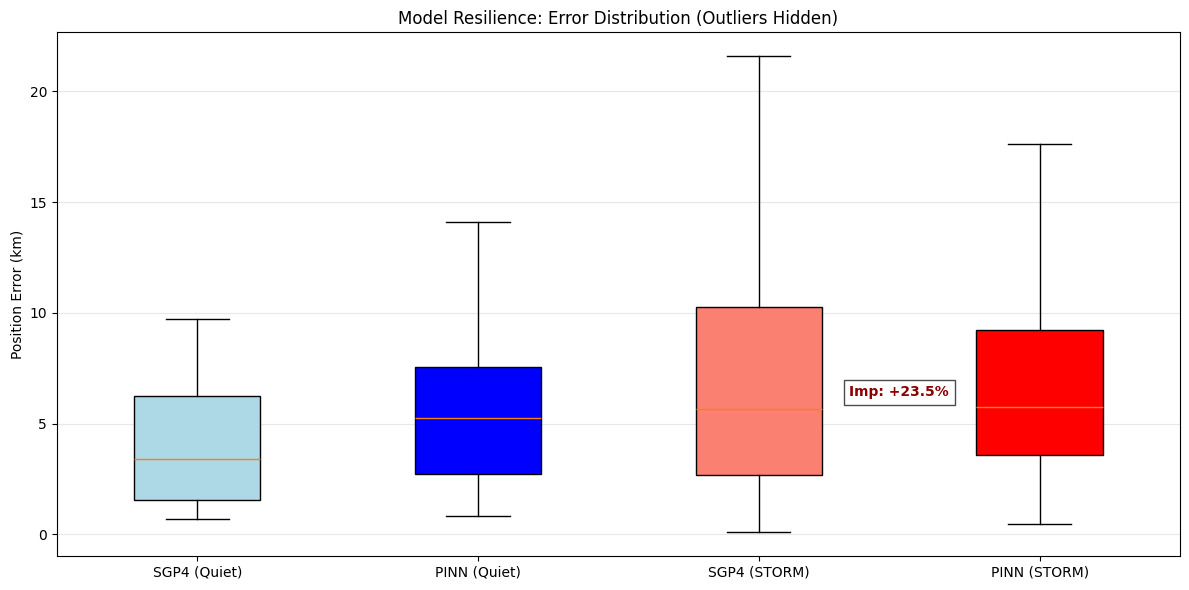
\includegraphics[width=\columnwidth]{figures/distribution.png}
\caption{Error-distribution comparison showing tail compression under storm conditions.}
\label{fig:error-distribution}
\end{figure}

The key operational benefit is tail-risk reduction: under severe storms, the model compresses extreme miss-distance spread from approximately 28 km to 21 km. This substantially reduces reacquisition search space and improves downstream conjunction triage during active storm windows \cite{parker2024satellite,kang2025solar}.

\subsection{Scientific Discovery: Persistent +5.5 m/s Bias}
Beyond prediction accuracy, learned residuals expose a stable radial correction of approximately $+5.5$ m/s for Starlink-3321. The consistency of this offset across samples suggests a systematic model-data mismatch rather than stochastic noise. In our interpretation, the network is compensating for degraded or lagging drag characterization in public-element handling, effectively acting as a diagnostic layer over legacy propagation \cite{dallinger2025cov,dey2024improving}.

\begin{figure}[H]
\centering
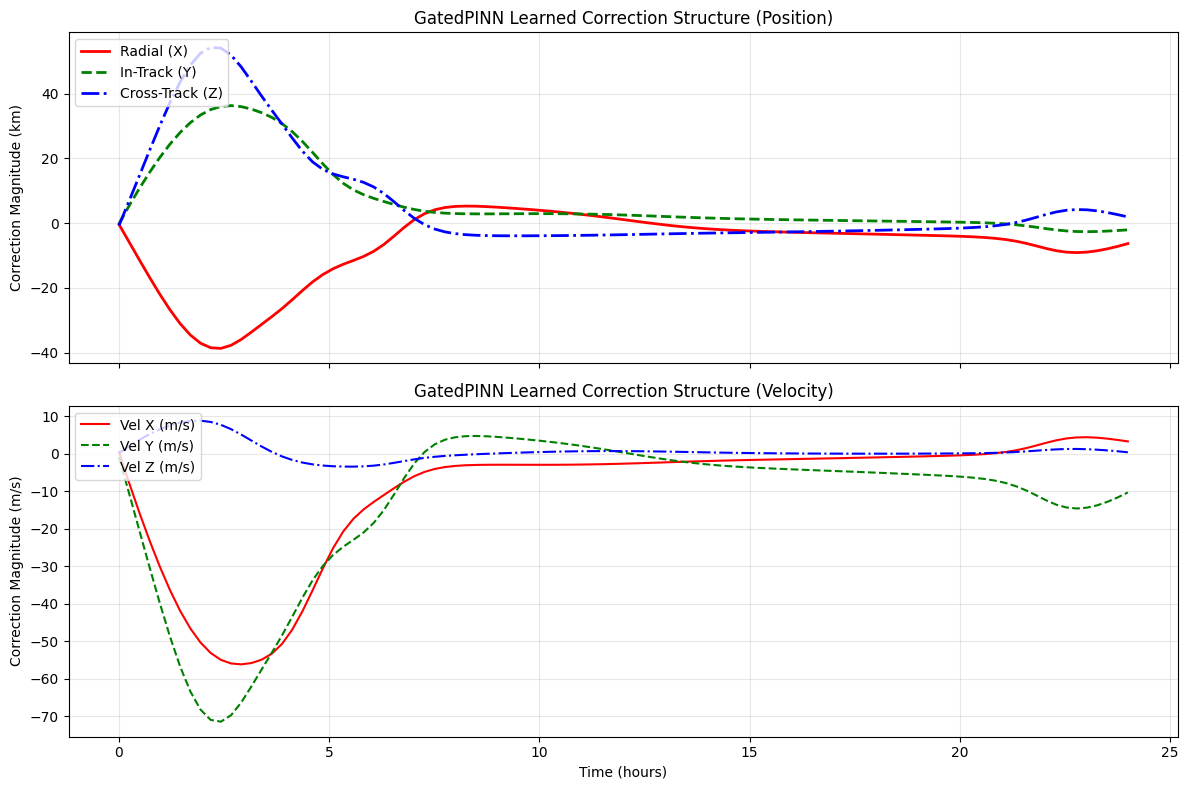
\includegraphics[width=\columnwidth]{figures/learned_correction.png}
\caption{Learned residual correction profile highlighting the persistent radial velocity bias component.}
\label{fig:learned-correction}
\end{figure}

\subsection{Conjunction Case Study and Risk Labeling}
In a representative close-approach scenario (January 12, 2022), the corrected trajectory preserves orbital geometry while shifting along-track state enough to alter covariance overlap behavior. The Mahalanobis classifier is therefore more informative than raw miss distance alone, because it captures both mean separation and anisotropic uncertainty in the encounter frame \cite{sanjuan2021uncertainty,li2025density}. This supports the use of G-PINN outputs as operational inputs to risk-prioritized maneuver planning.

\begin{figure}[H]
\centering
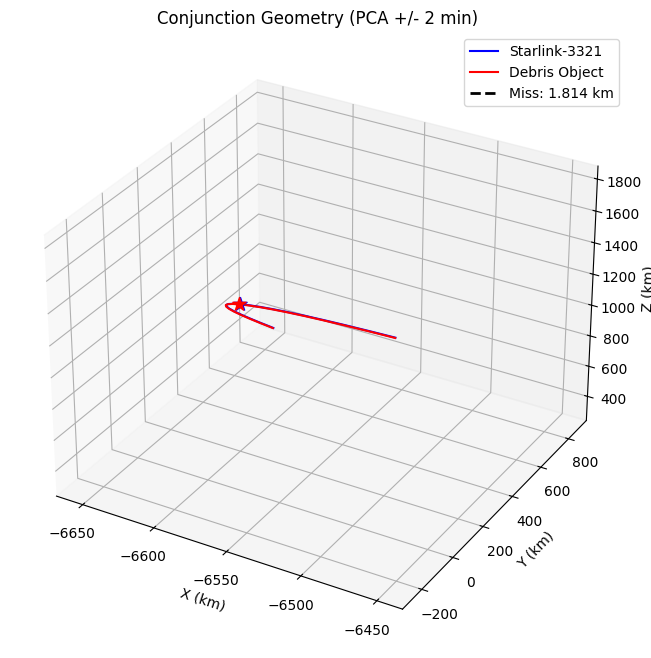
\includegraphics[width=\columnwidth]{figures/trajectory.png}
\caption{Corrected orbital trajectory evolution for the conjunction case study.}
\label{fig:trajectory-case}
\end{figure}
